\documentclass[tikz,border=7pt]{standalone}
\usepackage{amsmath}
\usepackage{pgfplots}
\usepgfplotslibrary{polar}
\pgfplotsset{compat=1.18}
\definecolor{ink}{HTML}{17324D}
\definecolor{accent}{HTML}{0F766E}
\definecolor{gold}{HTML}{C28524}
\begin{document}
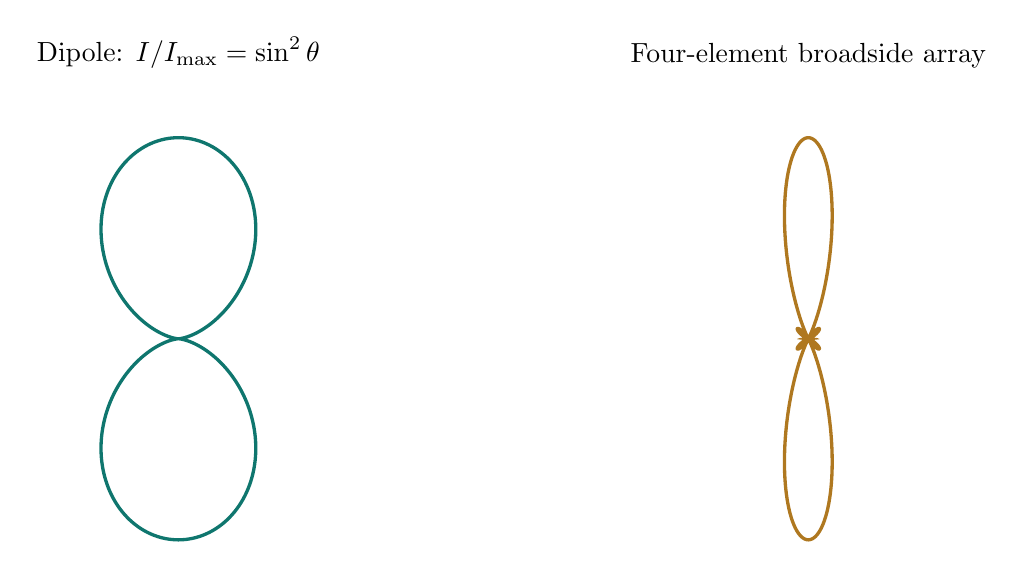
\begin{tikzpicture}
\begin{polaraxis}[
 at={(0cm,0cm)},anchor=west,
 width=7.2cm,height=7.2cm,
 axis lines=none,grid=both,
 xtick={0,45,...,315},ytick={0,.5,1},
 yticklabel style={font=\scriptsize},
 xticklabel style={font=\scriptsize},
 title={Dipole: $I/I_{\max}=\sin^2\theta$},
]
 \addplot[accent,very thick,domain=0:360,samples=361]
   {sin(x)^2};
\end{polaraxis}
\begin{polaraxis}[
 at={(8cm,0cm)},anchor=west,
 width=7.2cm,height=7.2cm,
 axis lines=none,grid=both,
 xtick={0,45,...,315},ytick={0,.5,1},
 yticklabel style={font=\scriptsize},
 xticklabel style={font=\scriptsize},
 title={Four-element broadside array},
]
 \addplot[gold!90!black,very thick,domain=0:360,samples=721]
   {(4+6*cos(180*cos(x))+4*cos(360*cos(x))+2*cos(540*cos(x)))/16};
\end{polaraxis}
\end{tikzpicture}
\end{document}
